\subsection{Admin Page}
The admin page is divided into three sections: “search”, “user details” and “update user details”. Upon
entering the page, only the “search” section will be filled.\\

The admin page allows to search for users via email. The selector is filled automatically with the emails
of all the registered users. Once the email of the user has been specified, by clicking on the “Search”
button, the two following sections (“user details” and “update user details”) are automatically filled with
the information on the users. In particular, in the section “user details” is reported a table with the user
email, first name, last name and role.\\ 

The section “update user details” contains a form, automatically filled with the data on the searched
user. The admin can update such data. They can then click on either the button “update” which
updates the user details, or the button “delete” which deletes the user from the database, revoking
their possibility to login and therefore to access reserved areas of the website.

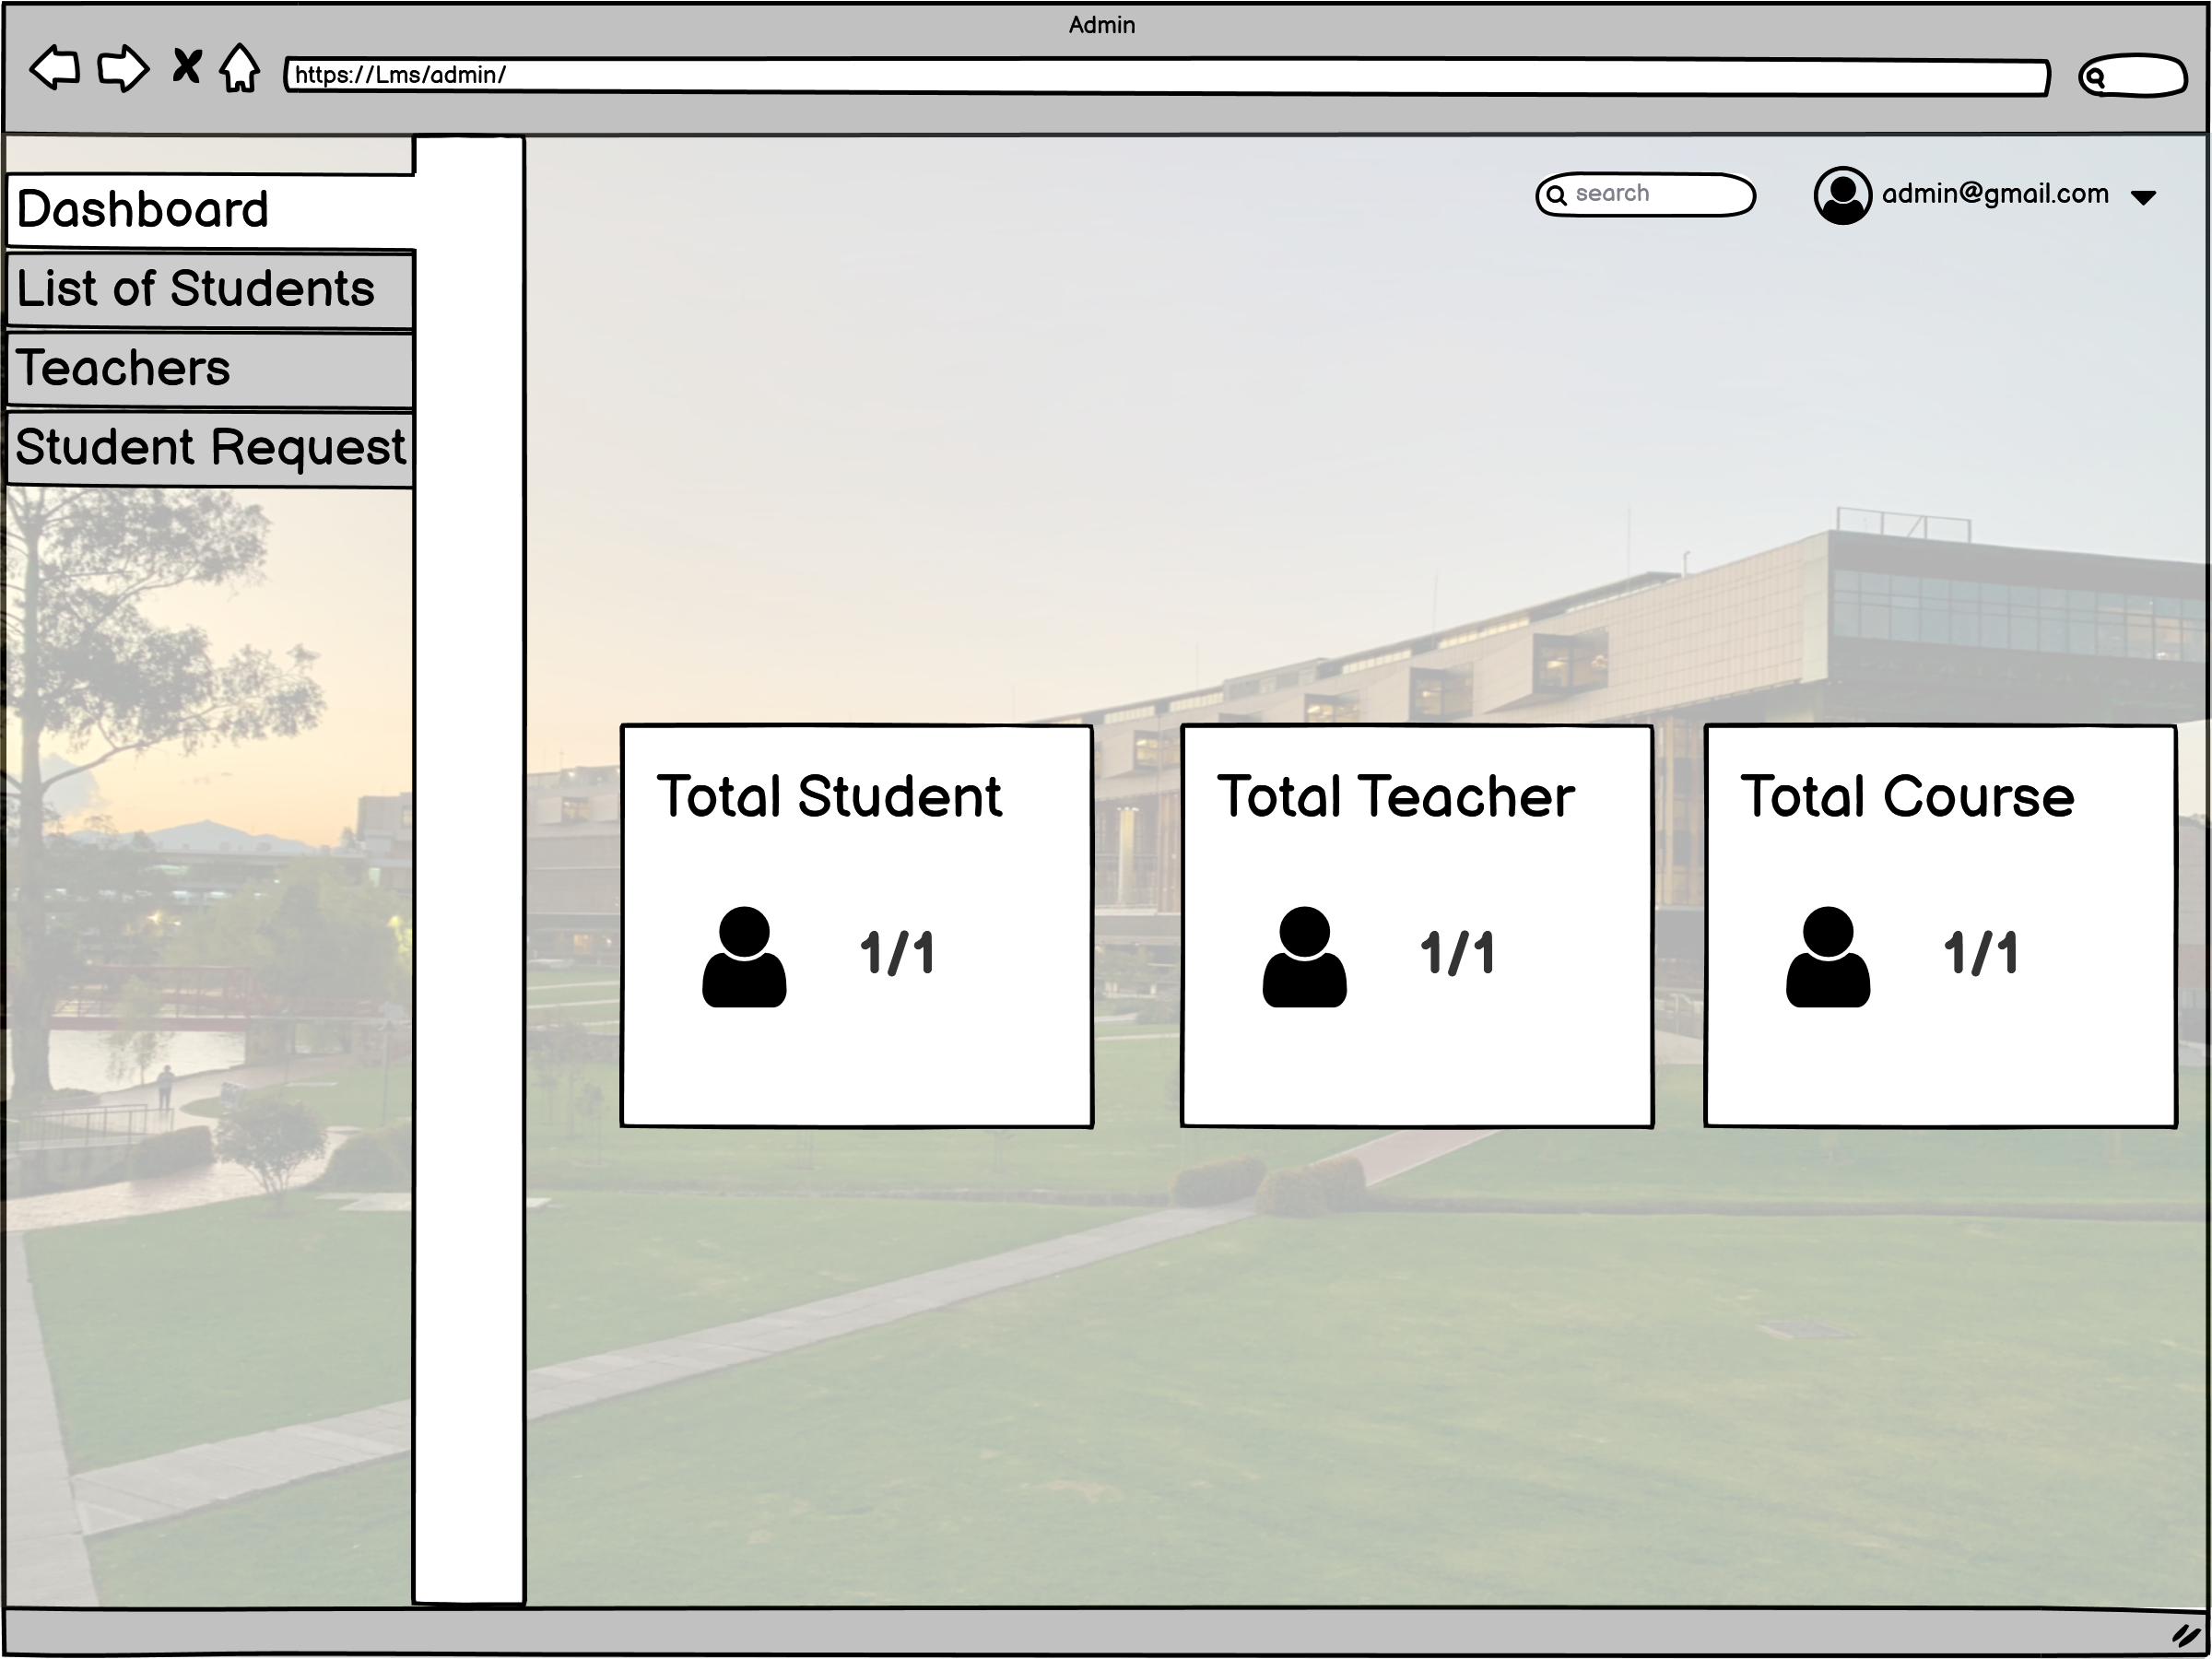
\includegraphics[width=\columnwidth]{images/Admin Page.png}